\section{Vorlesung 3: Systemmodellierung mit Petrinetzen}

\subsection*{Was ist ein Petrinetz?}

Auf diese Frage gibt es viele Antworten, die sich zwar recht unterschiedlich anhören, aber alle zutreffen (\sa \cite{des01}).

\begin{itemize}
	\item \textbf{Ein graphisches Modell:} Die visuelle Darstellung von Petrinetzen trägt dazu bei, Strukturen verteilter Systeme zu verstehen.
\end{itemize}


\begin{figure}[!htbp]
	\centering
	\scalebox{0.8}{
		\petrinetz{ 
			\node[place, tokens=3, label=above:\small{verfügbar}] (place1) at (2,2) {}; 
			\node[place, tokens=0, label=below:\small{leer}] (place2) at (2,-2) {}; 
			\node[place, tokens=1, label=above:\small{bereit für Münzeinwurf}] (place3) at (6,2) {}; 
			\node[place, tokens=0, label=below:\small{bereit zur Ausgabe}] (place4) at (6,-2) {}; 
			\node[place, tokens=0, label=right:\small{Münze halten}] (place5) at (10,0) {}; 
			
			\node[transition,label=left:\small{auffüllen}] (trans1) at (0,0) {}; 
			\node[transition,label=left:\small{ausgeben}] (trans2) at (4,0) {}; 
			\node[transition,label=right:\small{\ \ \ Münze einwerfen}] (trans3) at (8,2) {}; 
			\node[transition,label=below:\small{Münze zurückweisen}] (trans4) at (8,0) {};
			\node[transition,label=right:\small{\ \ \ Münze annehmen}] (trans5) at (8,-2) {};
			
			\draw 
			(trans1)edge[post, bend left=30](place1) 
			(trans2)edge[post, bend left=30](place2) 
			(place2)edge[post, bend left=30](trans1) 
			(place1)edge[post, bend left=30](trans2) 
			(place3)edge[pre, bend right=30](trans2) 
			(place3)edge[post](trans3) 
			(trans3)edge[post, bend left=30](place5) 
			(place5)edge[post](trans4) 
			(place5)edge[post, bend left=30](trans5) 
			(place4)edge[pre](trans5) 
			(trans4)edge[post, bend left=30](place3) 
			(place4)edge[post, bend left=30](trans2);
		}
	}
	\caption{Typisches Beispiel für ein Petrinetz: Ein Warenautomat}
	\label{fig:V3-Keksautomat}
\end{figure}

In Abbildung~\ref{fig:V3-Keksautomat} sind zwei Komponenten eines Warenautomaten erkennbar: die Steuerung (rechts) und der physische Automat (links). Neben dieser strukturellen Perspektive wird auch das Verhalten durch den Markenfluss visualisiert, dazu später. Der Warenautomat wird in der Videovorlesung näher erklärt.

\begin{itemize}
	\item \textbf{Ein mathematisches Modell:} Die formale Struktur eines Petrinetzes wird genutzt, um Zusammenhänge zwischen Eigenschaften auszudrücken und zu beweisen. Diese Eigenschaften können sich auf die Struktur eines Netzes und auf sein Verhalten beziehen.	
	
	Ein Petrinetz kann man definieren als $$N = (S, T, F, m_{0})$$ wobei gilt:
	\begin{itemize}
		\item $S$ ist die Menge der Stellen,
		
		\item $T$ ist die Menge der Transitionen,
		
		\item $F$ ist die Menge der Kanten, die jeweils eine Stelle mit einer Transition oder eine Transition mit einer Stelle verbinden (Kantenmenge),
		
		\item $m_{0}$ ist die Anfangsmarkierung, die die anfängliche Verteilung der Marken auf den Stellen beschreibt.
	\end{itemize}
	
	\item \textbf{Eine informatische Sprache:} Als formale Eingabe für Analyseprogramme, die oft die zuvor genannten formalen Zusammenhänge ausnutzen, dienen Petri\-netze der systematischen Überprüfung von Eigenschaften der von ihnen model\-lierten Systeme.
\end{itemize}


\subsection*{Elemente eines Petrinetzes}

Abbildung~\ref{fig:grundelemente_petrinetze} zeigt eine Zusammenfassung der Elemente von Petrinetzen.

\begin{figure}[!htbp]
	\begin{addmargin*}[0cm]{-\marginparwidth}
	\begin{addmargin*}[0cm]{-\marginparsep}
		\centering
		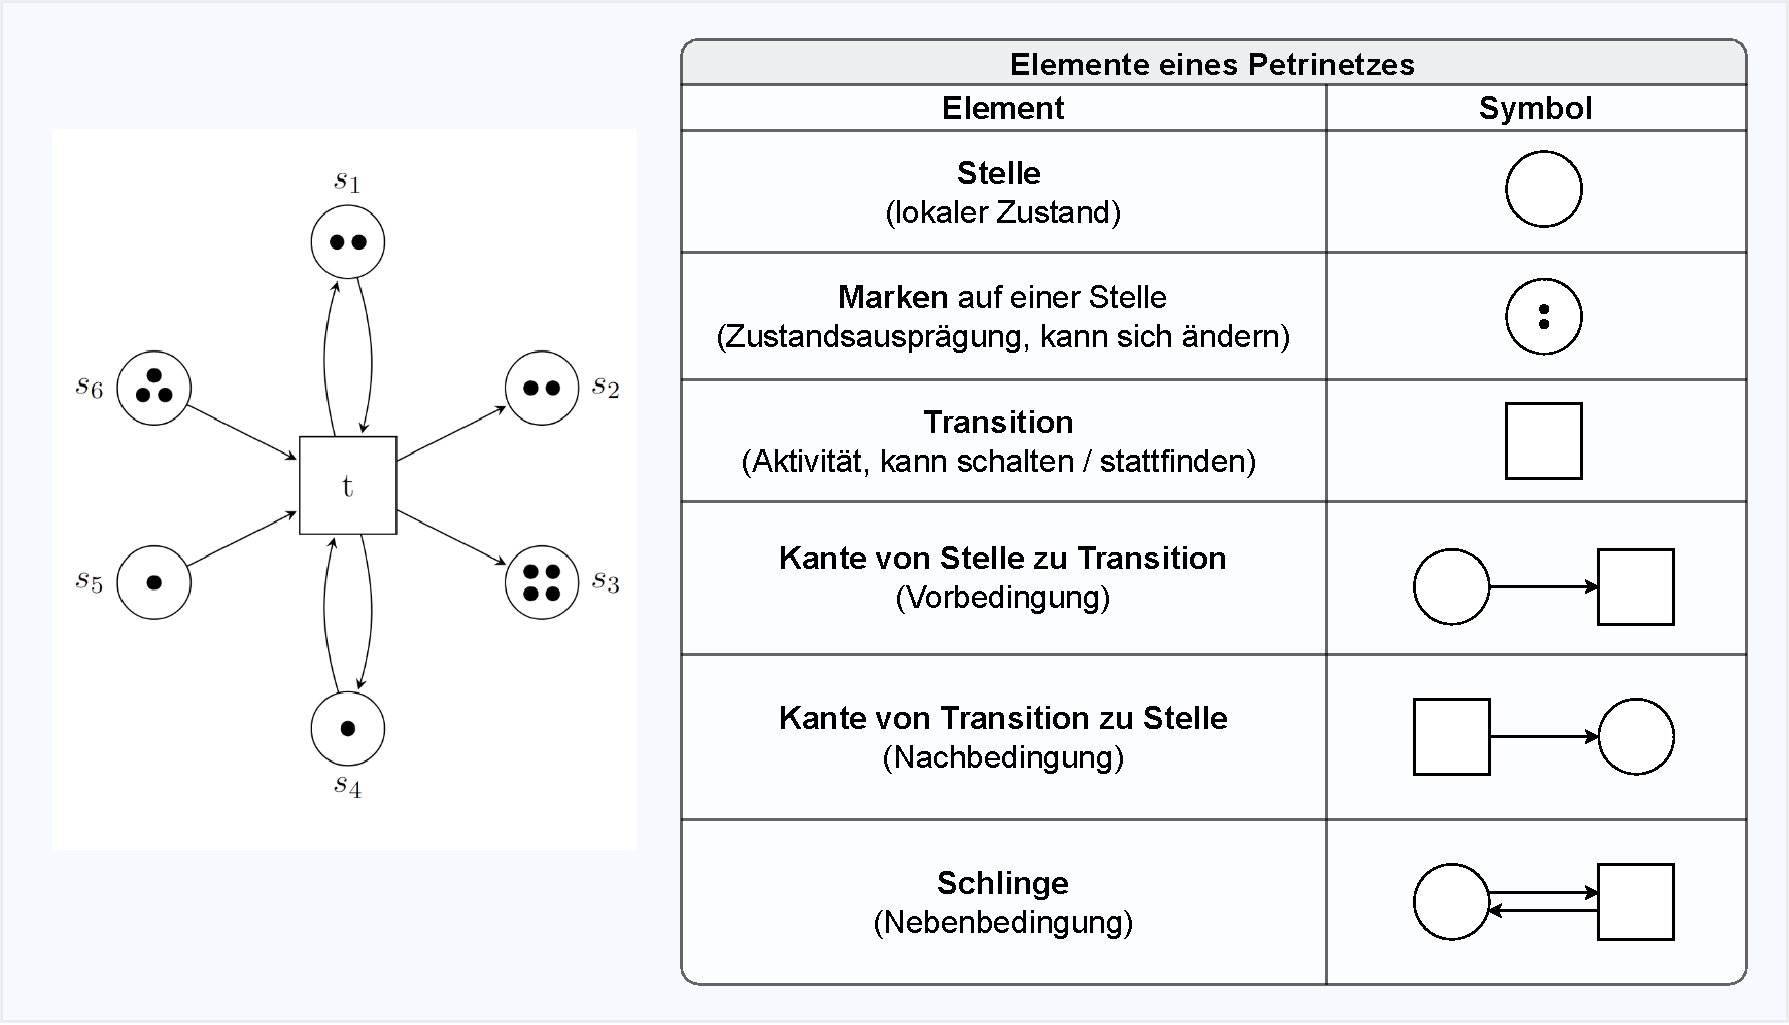
\includegraphics[width=\linewidth]{Bilder/Kapitel-5/grundelemente_petrinetze.pdf}
		\caption{Elemente von Petrinetzen}
		\label{fig:grundelemente_petrinetze}
	\end{addmargin*}
	\end{addmargin*}
\end{figure}

\minisec{Stellen}

Sie haben Stellen bereits in Petrinetzen kennengelernt, die Abläufe modellieren. 
\marginline{Stellen in Ablaufmodellen}
Dort repräsentieren sie Bedingungen, die unmittelbare kausale Abhängigkeiten von Aktionen darstellen. Jede derartige Bedingung kann unerfüllt oder erfüllt sein und gehört (mit Ausnahme von Anfang und Ende) stets zu einer Transition, nach deren Schalten sie erfüllt ist und zu einer Transition, deren Voraussetzung sie ist.

Nutzt man Petrinetze als Systemmodelle, können Stellen viel mehr ausdrücken. 
\marginline{Stellen im Systemmodell}
Es können mehrere Kanten zu einer Stelle führen, und es können mehrere Kanten von einer Stelle ausgehen und dadurch Alternativen dargestellt werden. Zudem kann eine Stelle auch mehr als nur zwei mögliche Zustände (unmarkiert / markiert bzw. unerfüllte Bedingung / erfüllte Bedingung) haben, denn sie kann auch mehr als eine Marke tragen. Dies kommt zwar in den meisten Modellen nur selten vor, aber ist zur Modellierung von mehrfach vorhandenen Ressourcen nützlich. Oder auch einfach dafür, denkbare Fehlerfälle (zum Beispiel unerwünschtes Überschreiben einer Variable oder Überlaufszenarien) formulieren zu können, auch wenn diese bei Modellen korrekter Systeme nicht vorkommen.


\minisec{Markierungen}

Um Verhalten eines Petrinetzes zu modellieren, benötigen wir Markierungen. Anschaulich ist eine Markierung eine Verteilung von Marken auf Stellen. Formal ist eine Markierung definiert als eine Abbildung $m: S \rightarrow \mathbb{N}_0$, die jeder Stelle $ s $ aus der Stellenmenge $S$ die natürliche Zahl $ m(s) $ zuweist. Diese Zahl $ m(s) $ gibt an, wie viele Marken sich auf der Stelle $ s $ befinden.

Wenn die Stellen (zum Beispiel durch Indizes der Form $ s_1, \ldots, s_k$ oder alphabetisch $A, B, C, \ldots$) geordnet sind, dann kann man eine Markierung $m$ als Vektor

$$ \underline{m} =
\begin{pmatrix}
	a_1 \\ \vdots \\ a_k
\end{pmatrix}
$$

schreiben, wobei $a_i$ die Zahl der Marken auf der $i$-ten Stelle ist.

\begin{figure}[!htbp]
	\centering
	\begin{minipage}[c]{.45\textwidth} 
		\centering
		\scalebox{0.8}{
			\petrinetz{
				% Places
				\node[place, tokens=1,label=left:$s_1$] (place1) at (2,0) {};
				\node[place, tokens=0,label=left:$s_2$] (place2) at (6,-2) {};
				\node[place, tokens=0,label=left:$s_3$] (place3) at (6,2) {};
				
				% Transitions
				\node[transition] (trans1) at (8,0) {};
				\node[transition] (trans2) at (4,0) {};
				
				% Edges
				\draw
				(place1) edge[post, bend left=15] (trans2)
				(place1) edge[pre, bend right=15] (trans2)
				(trans2) edge[post] (place2)
				(place2) edge[post] (trans1)
				(trans1) edge[post] (place3)
				(place3) edge[pre] (trans2);
			}
		}
		\vspace{1em}
		
		\textbf{$m_0$}\\
		~\\
		$m_0(s_1)=1$, $m_0(s_2)=0$, $m_0(s_3)=0$\\
		~\\
		$\underline{m_0}=
		\begin{pmatrix}
			1 \\ 0 \\ 0
		\end{pmatrix}$
	\end{minipage}
	\begin{minipage}[c]{.05\textwidth} 
		\centering
		{\color{FernUni-MI-green}\rule{1pt}{90mm}} % senkrechte farbige Linie
	\end{minipage}
	\begin{minipage}[c]{.45\textwidth}
		\centering
		\scalebox{0.8}{
			\petrinetz{
				% Places
				\node[place, tokens=1,label=left:$s_1$] (place1) at (2,0) {};
				\node[place, tokens=5,label=left:$s_2$](place2) at (6,-2) {};
				\node[place, tokens=7,label=left:$s_3$] (place3) at (6,2) {};
				
				% Transitions
				\node[transition] (trans1) at (8,0) {};
				\node[transition] (trans2) at (4,0) {};
				
				% Edges
				\draw
				(place1) edge[post, bend left=15] (trans2)
				(place1) edge[pre, bend right=15] (trans2)
				(trans2) edge[post] (place2)
				(place2) edge[post] (trans1)
				(trans1) edge[post] (place3)
				(place3) edge[pre] (trans2);
			}
		}
		\vspace{1em}
		
		\textbf{$m_7$}\\
		~\\
		$m_7(s_1)=1$, $m_7(s_2)=5$, $m_7(s_3)=7$\\
		~\\
		$\underline{m_7}=
		\begin{pmatrix}
			1 \\ 5 \\ 7
		\end{pmatrix}$
	\end{minipage}
	\caption{Beispiele für Markierungen}
	\label{fig:}
\end{figure}


Markierungen modellieren globale Zustände, konstituiert aus den lokalen Zuständen der einzelnen Stellen.

\minisec{Transitionen}

Wenn ein Petrinetz ein System darstellt, 
\marginline{Transitionen in Ablauf- und Systemmodellen}
dann modellieren Transitionen Aktivitäten. Wird ein Petrinetz zur Beschreibung eines Ablaufs verwendet, dann modellieren Transitionen Aktionen; die zugehörigen Aktivitäten bzw. die Transitionen eines System\-modells findet man dann meist als Label.


\minisec{Kanten und Markenspiel}

Bevor die Semantik, also die Schaltregel, in einer späteren Vorlesung formal definiert wird, sei hier für kleine Beispiele ein Spezialfall angegeben:

Wir betrachten ein Petrinetz $N=(S,T,F)$. 
\sttpkapitelverweis{Vorgriff Schaltregel (Definition~5.9)}{S.~\pageref{text:schaltregel}}
Eine Transition $t$ kann schalten, wenn jede Stelle $s$ mit $(s,t) \in F$ (wenigstens) eine Marke trägt. Wenn $t$ schaltet, wird von jeder dieser Stellen eine Marke entfernt und auf jeder Stelle $s$ mit $(t,s) \in F$ eine Marke hinzufügt, sodass immer wieder neue Markierungen erreicht werden. In einfachen Fällen entsteht dadurch ein "`Markenfluss"', der oft dem Kontrollfluss des modellierten Systems entspricht.


\subsection*{Deterministische Petrinetze}

Jede erreichbare Markierung kann keine, eine oder mehrere Transitionen aktivieren. Durch das Schalten einer Transition können neue Transitionen aktiviert werden. Es kann aber auch sein, dass eine andere, zuvor aktivierte Transition danach nicht mehr aktiviert ist, wenn nämlich eine von ihr benötigte Marke konsumiert wurde. Dieser Fall wird bezeichnet als 
\begin{itemize}
	\item Auswahl (zu welcher Transition geht die Marke?),
	\item Konflikt (zwei Transitionen „streiten“ um die Marke) oder
	\item Nichtdeterminismus (verschiedene Fortsetzungen sind möglich, es wurde keine spezifiert).
\end{itemize}

\begin{figure}[!htbp]
	\centering
	\scalebox{0.6}{
		\petrinetz{
			\draw[colDummyLine](-1,0) -- (19,0);
			
			% Places
			\node[place, tokens=0, label=left:$B$]  (place1) at (1.5,2.6) {}; 
			\node[place, tokens=1, label=below:$A$] (place2) at (1.5,-2.6) {}; 
			\node[place, tokens=0, label=right:$C$] (place3) at (6,0) {}; 
			\node[place, tokens=0, label=left:$G$]  (place4) at (12,0) {}; 
			\node[place, tokens=0, label=above:$F$] (place5) at (16.5,2.6) {}; 
			\node[place, tokens=1, label=below:$E$] (place6) at (16.5,-2.6) {}; 
			\node[place, tokens=0, label=above:$D$] (place7) at (9,2.6) {}; 
			\node[place, tokens=0, label=below:$H$] (place8) at (9,-2.6) {};
			
			% Transitions
			\node[transition, label=left:$a$]  (trans1) at (0,0) {}; 
			\node[transition, label=above:$b$] (trans2) at (4.5,2.6) {}; 
			\node[transition, label=below:$c$] (trans3) at (4.5,-2.6) {}; 
			\node[transition, label=above:$e$] (trans4) at (13.5,2.6) {}; 
			\node[transition, label=below:$f$] (trans5) at (13.5,-2.6) {}; 
			\node[transition, label=right:$d$] (trans6) at (18,0) {};
			
			
			% Kanten
			\draw (trans1) edge[post, bend left=20] (place1) (place1) edge[post, bend left=20] (trans2) (trans2) edge[post, bend left=20] (place3) (place3) edge[post, bend left=20] (trans3) (trans3) edge[post, bend left=20] (place2) (place2) edge[post, bend left=20] (trans1) (trans2) edge[post] (place7) (place7) edge[post] (trans4) (trans5) edge[post] (place8) (place8) edge[post] (trans3) (trans4) edge[post, bend right=20] (place4) (place4) edge[post, bend right=20] (trans5) (trans5) edge[post, bend right=20] (place6) (place6) edge[post, bend right=20] (trans6) (trans6) edge[post, bend right=20] (place5) (place5) edge[post, bend right=20] (trans4);
		}
	}
	\caption{Ein deterministisches Petrinetz}
	\label{fig:v3-deterministisches_Petrinetz}
\end{figure}

Bei deterministischen Petrinetzen kommt Nichtdeterminismus nicht vor. Typischerweise haben deterministische Petrinetze keine Stellen mit mehreren ausgehenden Kanten -- jede Marke kann dann nur von höchstens einer Transition konsumiert werden.

Vorsicht! Determinismus bedeutet nicht, dass die Anfangsmarkierung bzw.\ dass jede erreichbare Markierung nur eine Transition aktiviert. Die Markierung in Abbildung~\ref{fig:v3-deterministisches_Petrinetz} aktiviert beispielsweise die Transitionen $a$ und $d$. Es gibt aber trotzdem nur einen Ablauf (der aber mehrere sequentielle Beobachtungen hat). In anderen Worten: Aktiviert in deterministischen Petrinetzen eine Markierung mehrere Transitionen, so sind diese \textbf{nebenläufig} aktiviert.

\pagebreak %%% für Druck

\subsection*{Nicht-deterministische Petrinetze}	

In einem nicht-determinstischen Petrinetz gibt es Transitionen, die durch Marken auf derselben Stelle aktiviert werden. Abbildung~\ref{fig:v3-nicht-deterministisches Petrinetz} zeigt ein solches Netz: Nach Schalten von $a$ und $d$ (nebenläufig) stehen die Transitionen $b$ und $e$ in Konflikt. Es kann nur eine der beiden Transitionen ausgeführt werden, während die andere dadurch deaktiviert wird.

\begin{figure}[!htbp]
	\centering
	\scalebox{0.6}{
		\petrinetz{
			\draw[colDummyLine](-1,0) -- (19,0); 
			
			% Places
			\node[place, tokens=0, label=left:$B$]  (place1) at (1.5,2.6) {}; 
			\node[place, tokens=1, label=below:$A$] (place2) at (1.5,-2.6) {}; 
			\node[place, tokens=0, label=right:$C$] (place3) at (6,0) {}; 
			\node[place, tokens=0, label=left:$G$]  (place4) at (12,0) {}; 
			\node[place, tokens=0, label=above:$F$] (place5) at (16.5,2.6) {}; 
			\node[place, tokens=1, label=below:$E$] (place6) at (16.5,-2.6) {}; 
			\node[place, tokens=1, label=above:$D$] (place7) at (9,0) {};
			%\node[place, tokens=1, label=below:$H$] (place8) at (8,-2.6) {};
			
			% Transitions
			\node[transition,label=left:$a$]   (trans1) at (0,0) {}; 
			\node[transition, label=above:$b$] (trans2) at (4.5,2.6) {}; 
			\node[transition, label=below:$c$] (trans3) at (4.5,-2.6) {}; 
			\node[transition, label=above:$e$] (trans4) at (13.5,2.6) {}; 
			\node[transition, label=below:$f$] (trans5) at (13.5,-2.6) {}; 
			\node[transition, label=right:$d$] (trans6) at (18,0) {};
			
			% Kanten
			\draw (trans1) edge[post, bend left=20] (place1) (place1) edge[post, bend left=20] (trans2) (trans2) edge[post, bend left=20] (place3) (place3) edge[post, bend left=20] (trans3) (trans3) edge[post, bend left=20] (place2) (place2) edge[post, bend left=20] (trans1) (trans2) edge[pre] (place7) (place7) edge[post] (trans4) (trans5) edge[post] (place7) (place7) edge[pre] (trans3) (trans4) edge[post, bend right=20] (place4) (place4) edge[post, bend right=20] (trans5) (trans5) edge[post, bend right=20] (place6) (place6) edge[post, bend right=20] (trans6) (trans6) edge[post, bend right=20] (place5) (place5) edge[post, bend right=20] (trans4);
		}
	}
	\caption{Nicht-deterministisches Petrinetz}
	\label{fig:v3-nicht-deterministisches Petrinetz}
\end{figure}


\subsection*{Komponenten und Lokalität}	

Abbildung~\ref{fig:v3-Komponenten-und-lokalitaet} zeigt mögliche Komponenten des Petrinetzes aus Abbildung~\ref{fig:v3-deterministisches_Petrinetz} (blaue Kreise). Elemente innerhalb derselben Komponente sind \textbf{lokal}. Beispiel: Transition $a$ und Stelle $C$ befinden sich in derselben Lokalität (obwohl sie nicht direkt mit einer Kante verbunden sind). Verbindungen zwischen Elementen aus unterschied\-lichen Komponenten können als \textbf{global} angesehen werden.

\begin{figure}[!htbp]
	\centering
	\scalebox{0.6}{
		\petrinetz{ 
			\draw[colDummyLine](-1,0) -- (19,0); 
			
			\fill[teal!70!blue, opacity=0.2] (3,0) circle (4); 
			\fill[teal!70!blue, opacity=0.2] (9,2.6) circle (1); 
			\fill[teal!70!blue, opacity=0.2] (9,-2.6) circle (1); 
			\fill[teal!70!blue, opacity=0.2] (15,0) circle (4);
			
			% Places
			\node[place, tokens=0, label=left:$B$]  (place1) at (1.5,2.6) {}; 
			\node[place, tokens=1, label=below:$A$] (place2) at (1.5,-2.6) {}; 
			\node[place, tokens=0, label=right:$C$] (place3) at (6,0) {}; 
			\node[place, tokens=0, label=left:$G$]  (place4) at (12,0) {}; 
			\node[place, tokens=0, label=above:$F$] (place5) at (16.5,2.6) {}; 
			\node[place, tokens=1, label=below:$E$] (place6) at (16.5,-2.6) {}; 
			\node[place, tokens=0, label=above:$D$] (place7) at (9,2.6) {}; 
			\node[place, tokens=0, label=below:$H$] (place8) at (9,-2.6) {};
			
			% Transitions
			\node[transition, label=left:$a$]  (trans1) at (0,0) {}; 
			\node[transition, label=above:$b$] (trans2) at (4.5,2.6) {}; 
			\node[transition, label=below:$c$] (trans3) at (4.5,-2.6) {}; 
			\node[transition, label=above:$e$] (trans4) at (13.5,2.6) {}; 
			\node[transition, label=below:$f$] (trans5) at (13.5,-2.6) {}; 
			\node[transition, label=right:$d$] (trans6) at (18,0) {};
			
			% Kanten
			\draw (trans1) edge[post, bend left=20] (place1) (place1) edge[post, bend left=20] (trans2) (trans2) edge[post, bend left=20] (place3) (place3) edge[post, bend left=20] (trans3) (trans3) edge[post, bend left=20] (place2) (place2) edge[post, bend left=20] (trans1) (trans2) edge[post] (place7) (place7) edge[post] (trans4) (trans5) edge[post] (place8) (place8) edge[post] (trans3) (trans4) edge[post, bend right=20] (place4) (place4) edge[post, bend right=20] (trans5) (trans5) edge[post, bend right=20] (place6) (place6) edge[post, bend right=20] (trans6) (trans6) edge[post, bend right=20] (place5) (place5) edge[post, bend right=20] (trans4);
		}
	}
	\caption{Komponenten und Lokalität}
	\label{fig:v3-Komponenten-und-lokalitaet}
\end{figure}
